%\chapter{Solar radiation in South Africa and load curve covering concept}\label{Solar power in South Africa}
%South Africa is one of the country with the highest potential for generating solar thermal electricity in the word. Figure \ref{DHI-DIF} shows  the daily sum of global irradiation in Aberdeen, United Kingdom and Upington, South Africa. The yearly share of diffuse irradiation in Aberdeen overlaps 60 \%. In winter month the share reaches 90 \%. The share in Upington is approximately 25 \% and is in total significantly higher than Aberdeen. The direct comparison shows also the difference of the solar irradiation between northern and southern hemisphere during the year. It is obviously, that the seasons are the other way around between both hemispheres.
\chapter{Solar radiation in South Africa and load curve covering}\label{Solar power in South Africa}
South Africa is among the countries with the greatest potential for generating solar thermal electricity. The percentage of total radiation that is diffuse in Aberdeen, United Kingdom is \SI{60}{\percent}; in winter months it can be as high as \SI{90}{\percent} (Figure \ref{DHI-DIF}). In Upington, South Africa, the diffuse share is \SI{25}{\percent} and total radiation is significantly higher than in Aberdeen. The seasonal differences between northern and southern hemispheres are evident.

%This chapter shows energy impact from the sun and how it is distributed in SA. Furthermore the chapter comprised the current situation of solar power plants in SA.
\begin{figure}[h!] % DHI-DFI
\centering
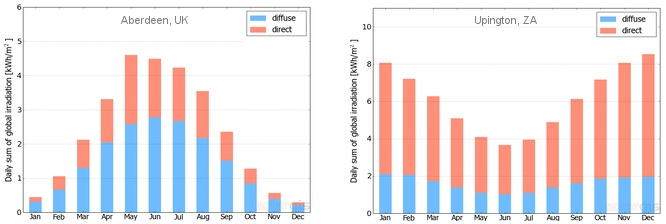
\includegraphics[width=1\linewidth]{FIG/DHI-DIF}
\caption[Long-term monthly variability of direct (DNI) and diffuse (DHI) irradiaton throughout the year for Aberdeen, UK and Upington, RSA.]{Long-term monthly variability of direct (DNI) and diffuse (DHI) irradiaton throughout the year for Aberdeen, UK and Upington, RSA \cite{SolarGIS2015}.}\label{DHI-DIF}
\end{figure} 
\section{Solar radiation}

%The most important solar radiation parameters for designing a solar power plant are here defined:
The solar radiation parameters most critical for power plant design are:
\begin{itemize}
%\item \textbf{GHI} (kWh/m\textsuperscript{2}/a or W/m\textsuperscript{2}): Global Horizontal Irradiance is the total amount of shortwave radiation received from above by a horizontal surface. It includes direct (beam) and a diffuse (scattered) irradiation. This value is of particular interest to PV or solar water heater with a fixed inclined angle.
\item \textbf{GHI} (\si{\kilo\watt\hour\per\squared\metre\year} or \si{\watt\per\squared\metre}): \emph{Global Horizontal Irradiance} is the total amount of shortwave radiation received from above by a horizontal surface. It includes direct (beam) and a diffuse (scattered) irradiation. This value is of particular interest when designing PV or solar water heater systems with a fixed inclined angle.
%\item \textbf{DNI} (kWh/m\textsuperscript{2}/a or W/m\textsuperscript{2}): Direct Normal Irradiance is the amount of solar radiation received per unit area by a surface that is always held perpendicular (or normal) to the rays that come in a straight line from the direction of the sun at its current position in the sky. Diffuse irradiation is totally excluded from the DNI. This quantity is of particular interest to  installations that track the position of the sun.
\item \textbf{DNI} (\si{\kilo\watt\hour\per\squared\metre\year} or \si{\watt\per\squared\metre}): \emph{Direct Normal Irradiance} is the amount of solar radiation received per unit area by a surface that is always held perpendicular (or normal) to the rays that come in a straight line from the direction of the sun at its current position in the sky. Diffuse irradiation is totally excluded from the DNI. This quantity is relevant for installations that track the position of the sun.
%\item \textbf{DHI} (kWh/m\textsuperscript{2}/a or W/m\textsuperscript{2}): Diffuse Horizontal Irradiance is the amount of radiation received per unit area by a surface that does not arrive on a direct path from the sun, but has been scattered by molecules and particles in the atmosphere and comes equally from all directions.
\item \textbf{DHI} (\si{\kilo\watt\hour\per\squared\metre\year} or \si{\watt\per\squared\metre}): \emph{Diffuse Horizontal Irradiance} is the amount of radiation received per unit area by a surface that does not arrive on a direct path from the sun, but has been scattered by molecules and particles in the atmosphere and comes equally from all directions.
\end{itemize}
%Furthermore is irradiance understood as instantaneous density of solar radiation incident on a given surface, typically expressed in W/m\textsuperscript{2} and irradiation is the sum of irradiance over a time period expressed in J/m\textsuperscript{2} or more commonly used in Wh/m\textsuperscript{2}. The connection between the solar radiation parameters is shown in Equation \ref{GL_GHI}.The angle $\theta_\text{z}$ is the angle between the direction of the sun and the zenith (directly overhead).
\emph{Irradiance} is understood as the instantaneous density of solar radiation incident on a given surface and is typically expressed in \si{\watt\per\squared\metre} and \emph{irradiation} is the sum of irradiance over a time period expressed in \si{\joule\per\squared\metre} or the more commonly used \si{\watt\hour\per\squared\metre}. The relationship between solar radiation parameters is shown by Equation \ref{GL_GHI}.The angle $\theta_\text{z}$ is the angle between the direction of the sun and the zenith (directly overhead).
\begin{align}
\text{GHI}=\text{DNI}\cdot\cos(\theta_{z})+\text{DHI}\label{GL_GHI}
\end{align}
%Figure\ref{irradiation} shows the solar GHI and the DNI data for the country. It is shown, that the ceiling value for GHI can be more than 2~300~kWh/m\textsuperscript{2}/a, whereas in some parts of the country the DNI  value attains about 2~900~kWh/m\textsuperscript{2}/a. This is significantly high than in the most regions worldwide, therefor SA is predestined for using solar technologies. The figure shows, that the southeastern coastline has predominantly the lowest irradiance values. The solar irradiation rise significant in the inland. The highest GHI can be find close to the Namibian boarder in the northeast of the country. The direct beam is also at highest in the western part of SA. The area around Springbok in the province Northern Cape has the highest DNI value of the country.
In South Africa, the ceiling for GHI is more than \SI{2300}{\kilo\watt\hour\per\squared\metre\year}, while in some parts of the country DNI is as high as \SI{2900}{\kilo\watt\hour\per\squared\metre\year} (Figure\ref{irradiation}), significantly higher than in most regions of the world. As such, solar power is South Africa is particularly well-suited to solar power. The highest GHI occurs close to the Namibian border in the northwest. The direct beam is also at its highest in western SA. The area around Springbok in Northern Cape province has the highest DNI.

%% Abbildung GHI und DNI
\begin{figure}[h!]
        \centering
        \begin{subfigure}[b]{0.5\textwidth}
                \centering
                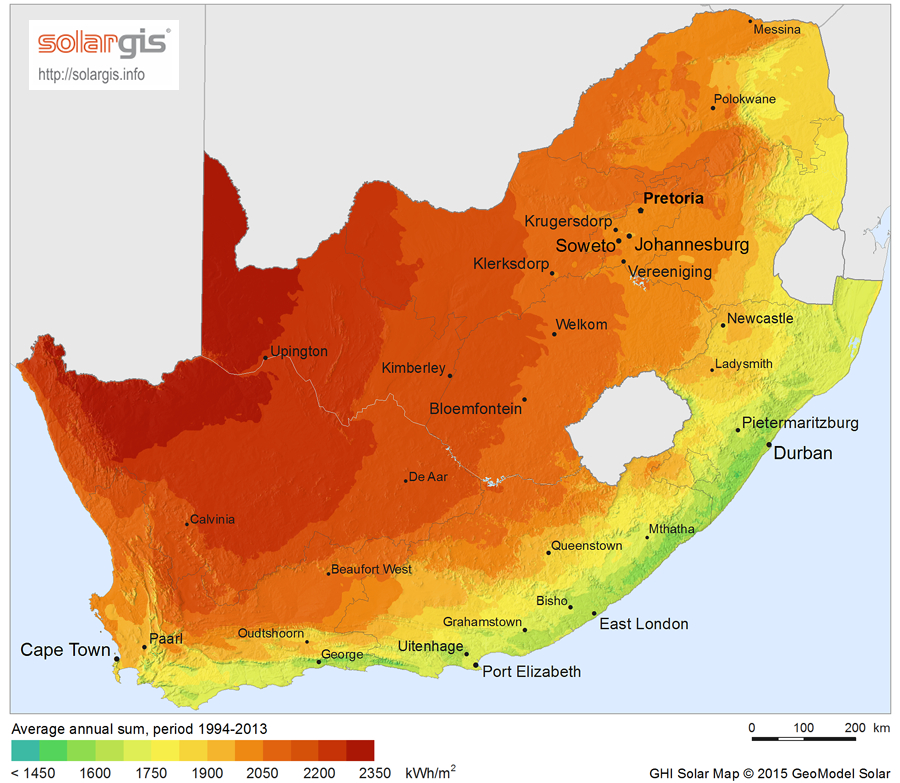
\includegraphics[width=0.95\textwidth]{FIG/SA_GHI}
                \caption{Global Horizontal Irradiation \cite{SolarGIS2015a}.}\label{fig:bild-links}
        \end{subfigure}%
        ~
        \begin{subfigure}[b]{0.5\textwidth}
                \centering
                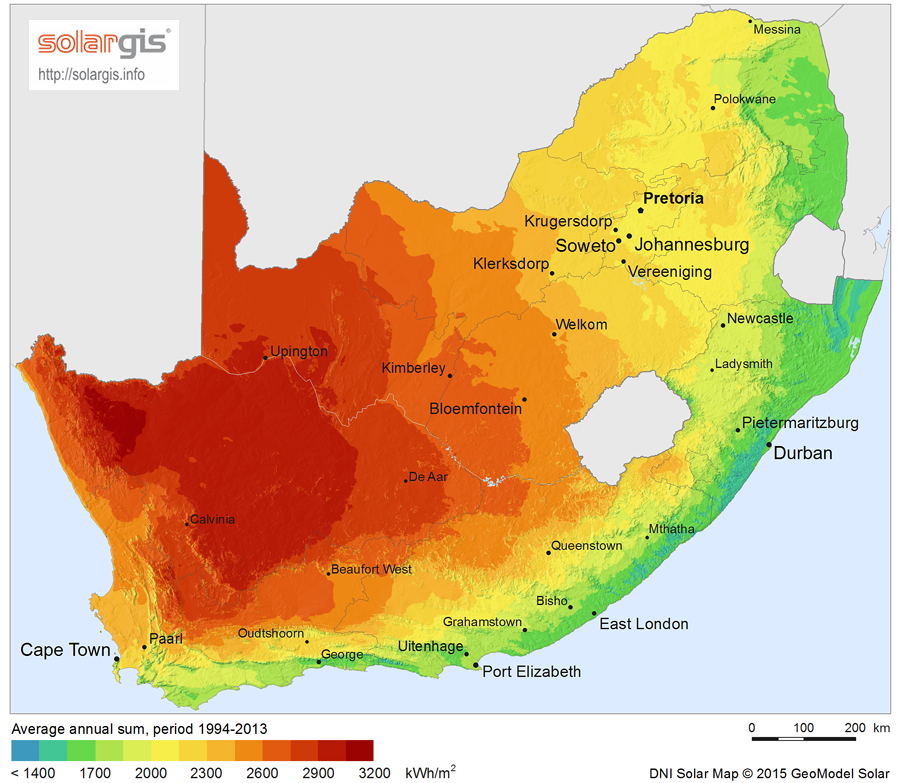
\includegraphics[width=0.95\textwidth]{FIG/SA_DNI}
                \caption{Direct Normal Irradiation \cite{SolarGIS2015b}.}\label{fig:bild-rechts}
        \end{subfigure}
        \caption{Solar radiation maps of South Africa.}\label{irradiation}
\end{figure}
\pagebreak
\section{Solar power plants in South Africa}

%South Africa started there expansion in the field of solar power plants in the first round of the Renewable Energy Independent Power Producer Procurement Program (REIPPPP) in 2011. Now in 2015 starts the fourth round of the REIPPPP. Figure \ref{Solar-map} shows the allocation of all solar power plants of the REIPPPP. PV-power plants are marked in yellow and CSP-power plants are marked in orange. The numbers in the single marks expose in which REIPPPP-Round it belongs.
South Africa's solar power expansion began with the first round of the Renewable Energy Independent Power Producer Procurement Program (REIPPPP) in 2011, and continues through to the fourth round of the REIPPPP in 2015. Figure \ref{Solar-map} shows the location of all REIPPPP solar power plants. Photovoltaic plants are marked in yellow and CSP plants are marked in orange. The numbers in the marks correspond to the applicable REIPPPP round.

\begin{figure}[h!] % Solar-map
\centering
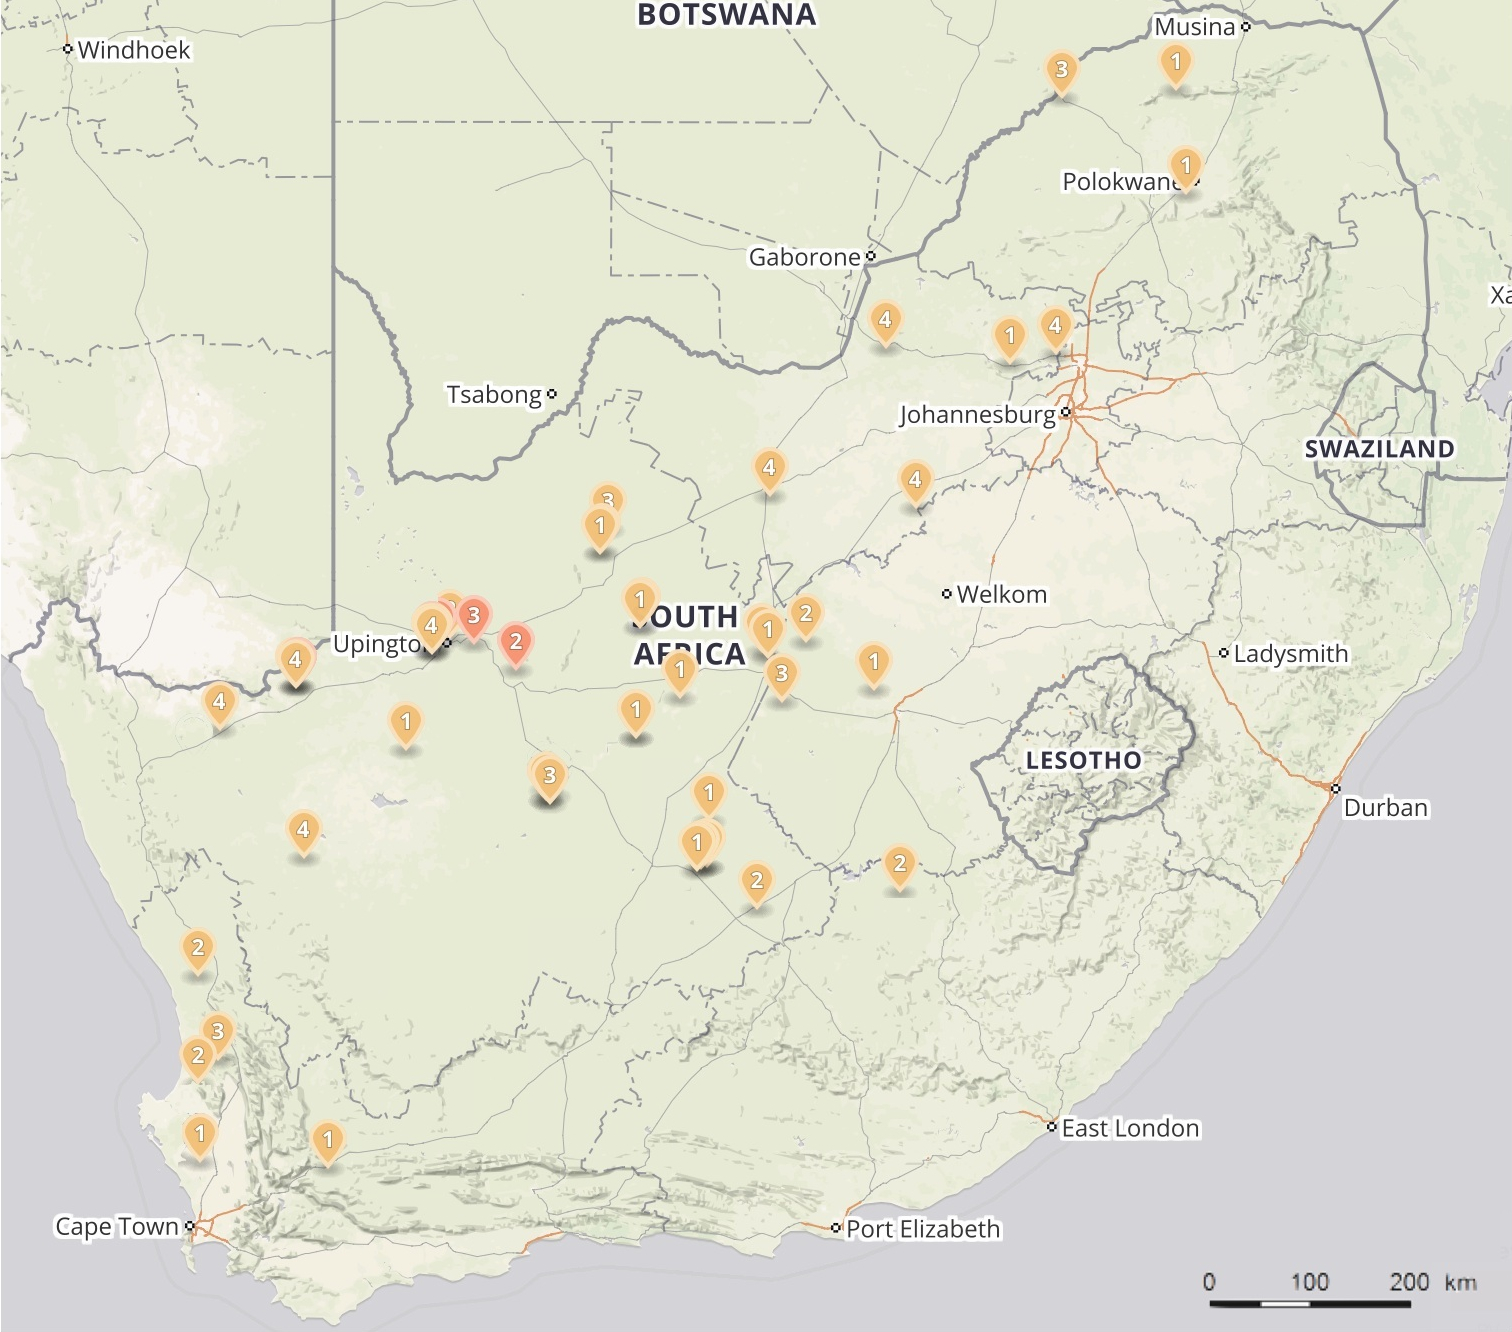
\includegraphics[width=1\linewidth]{FIG/Solar-map}
\caption[REIPPPP solar power plants in South Africa.]{REIPPPP solar power plants in South Africa \cite{Forder2015}.}\label{Solar-map}
\end{figure}

South Africa has 26 fully operational PV plants with a total capacity of \SI{1048.7}{\mega\watt}, a further seven with \SI{135.35}{\mega\watt} are under construction, four more with \SI{307.5}{\mega\watt} waiting to begin construction (approved and financed) and six more in approvals, planning and financing with a total capacity of \SI{415}{\mega\watt}. Of the total, 26 of 39 of the operational and planned plants are located in Northern Cape, five in the Western Cape, three each in the Free State and Limpopo and one each in Eastern Cape and the North-West Province \cite{Forder2015}.

%Mainly PV-power plants are allocated in the Northern Cape. So 26 of 39 of the operational and planed plants are located there. Five more in the Western Cape, three each in the provinces Free State and Limpopo and each one in Eastern Cape and the North-West Province. \cite{Forder2015}

%"KaXu Solar One" is the first fully operational CSP-plant in SA and is shown in Figure \ref{KaXu-solar-field}. It is using parabolic trough technology and a 2.5~h thermal energy storage for generating of 100~MW capacity electricity. The CSP-plants "Khi Solar One" and "Bokpoort CSP Project" with a capacity of each 50~MW are under construction. Further three CSP-plants are awaiting construction, they have all a capacity of each 100~MW. 
\emph{KaXu Solar One} is the first fully operational CSP plant in South Africa (Figure \ref{KaXu-solar-field}). It uses parabolic trough technology with \SI{2.5}{\hour} thermal energy storage for \SI{100}{\mega\watt} generating capacity. The CSP plants \emph{Khi Solar One} and \emph{Bokpoort CSP Project} with a capacity of \SI{50}{\mega\watt} each are now under construction. An additional three CSP plants, each with a generating capacity of \SI{100}{\mega\watt} are awaiting construction. 

%All six CSP-plants are located in the region around the cites to Upington or Pofadder in the Northern Cape. This region is predestined for CSP-plants, because it has high DNI (around~2~900~kWh/m\textsuperscript{2}/a) and a water connection through the Orange River. \cite{Forder2015}
All of the operating and planned CSP plants are located around Upington and Pofadder in the Northern Cape, a region particularly suited to CSP plants because of its high DNI (\SI{2900}{\kilo\watt\hour\per\squared\meter\year}) and its water access via the Orange River \cite{Forder2015}.

\begin{figure}[!h]
\centering
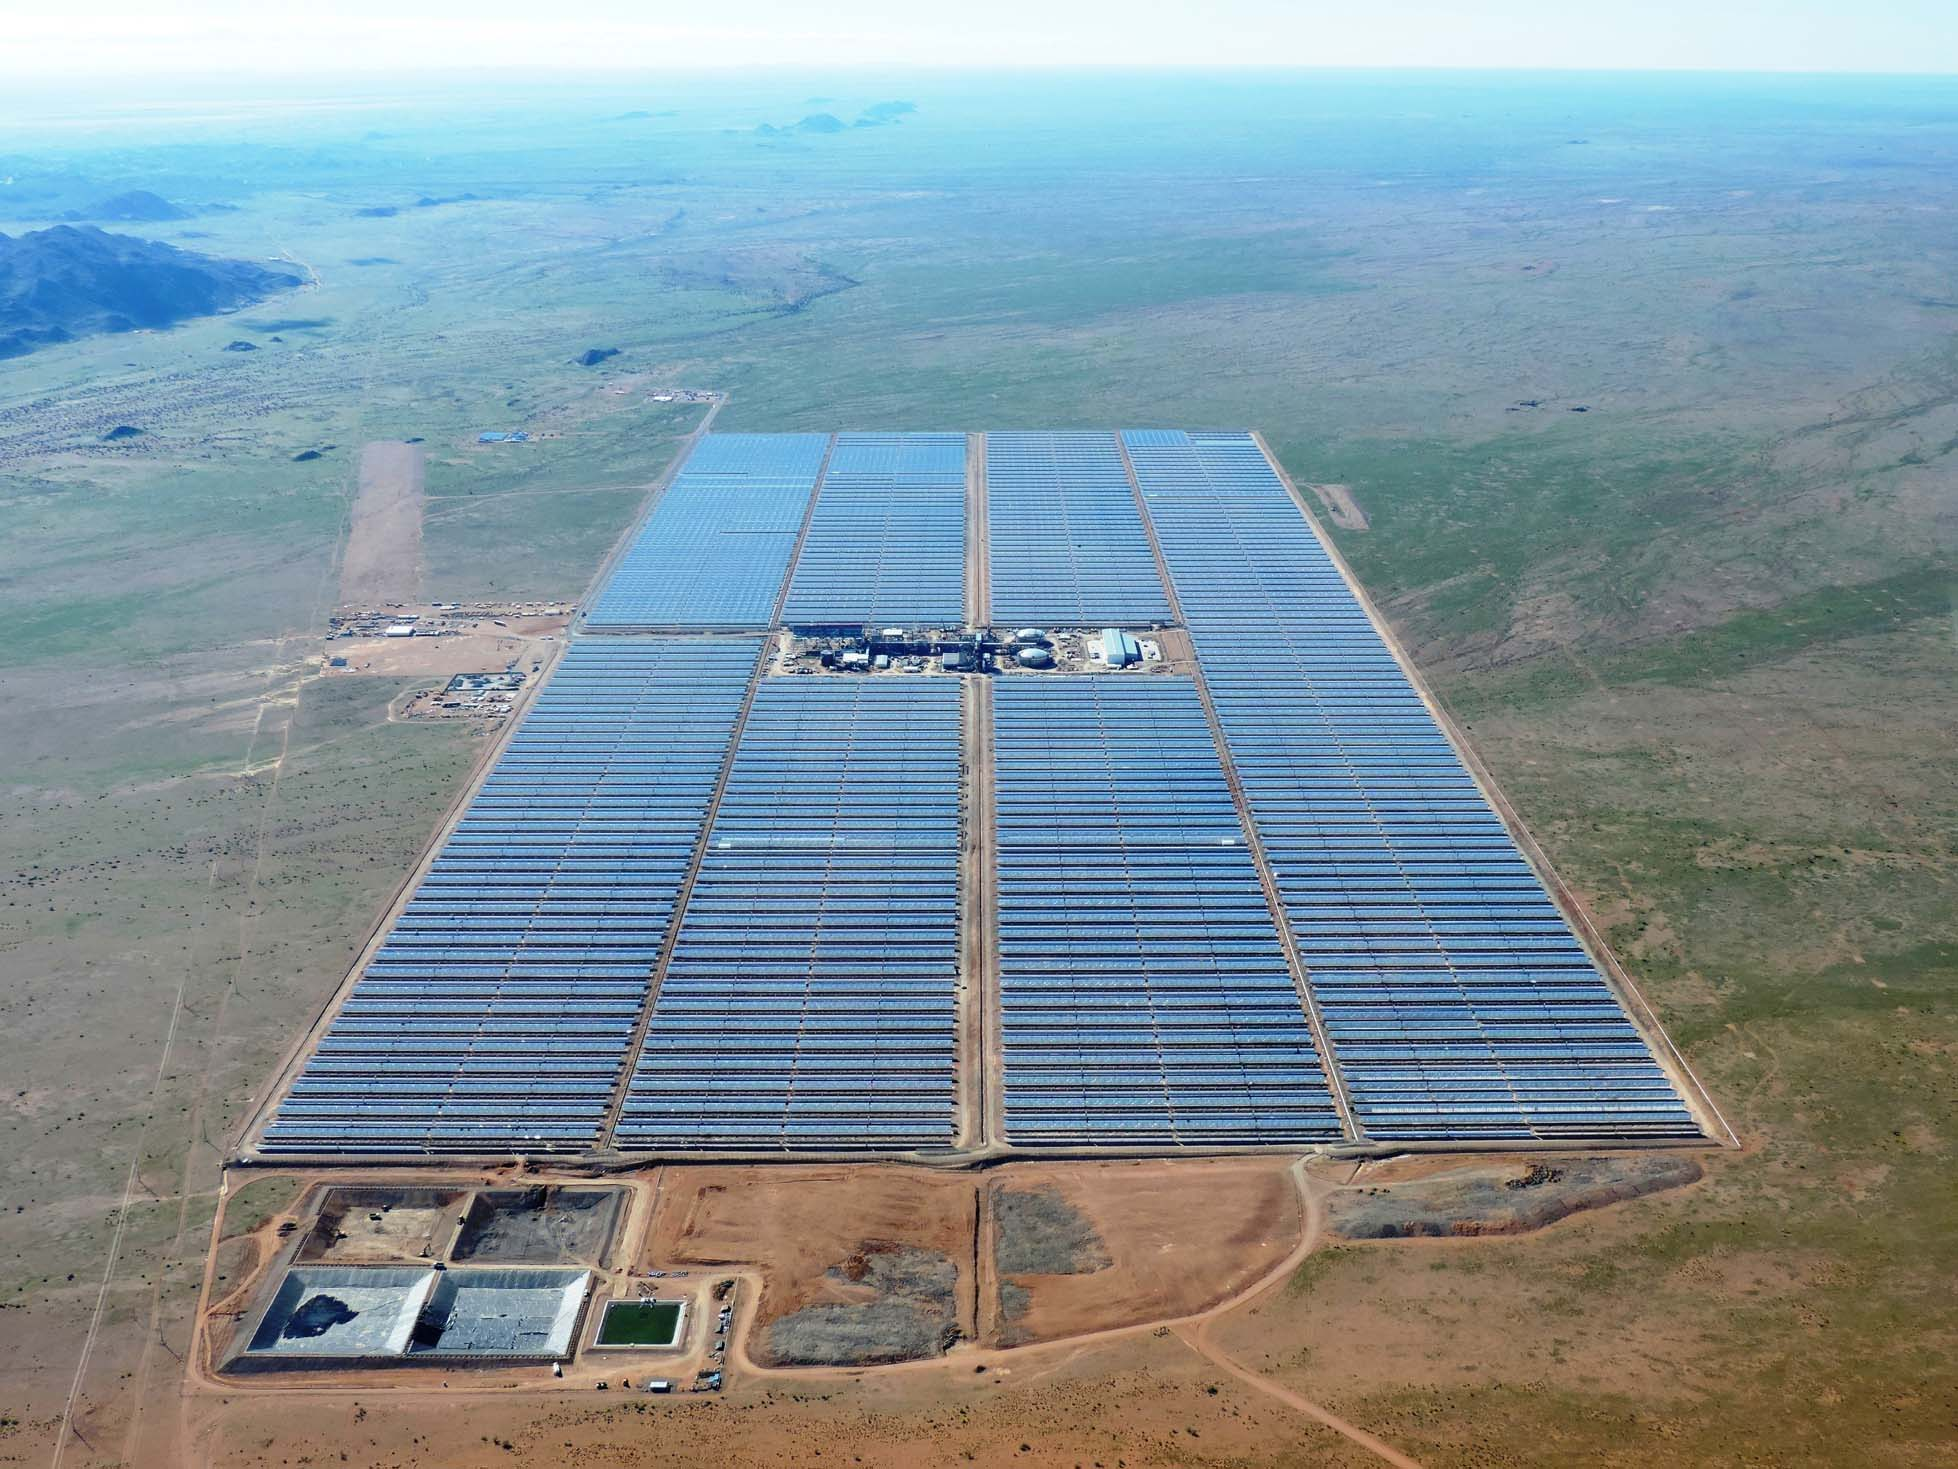
\includegraphics[width=1\linewidth]{FIG/KaXu-solar-field}
\caption[KaXu Solar One, a \SI{100\{\mega\watt} parabolic trough plant with 2.5 hours of thermal storage in molten salts.]{KaXu Solar One, a \SI{100\{\mega\watt} parabolic trough plant with 2.5 hours of thermal storage in molten salts \cite{AbengoaSolar2015}.}\label{KaXu-solar-field}
\end{figure}

\pagebreak
